\documentclass{article}
\usepackage[utf8]{inputenc}
\usepackage[margin=3.0cm]{geometry}
\usepackage{minted}
\usepackage{amssymb}
\usepackage{amsthm}
\usepackage{amsmath}
\usepackage{graphicx}
\usepackage{bbm}
\usepackage{bm}
\usepackage[table]{xcolor}
\newcommand{\wo}{\mathbbm{w}}

\pdfinfo{
/Title (neural)
/Author (Felipe Salvatore)}
\setcounter{secnumdepth}{0}  


\title{Feed-forward neural network: backpropagation}
\author{Felipe Salvatore\\
\texttt{felipessalvador@googlemail.com}}
\begin{document}
\maketitle
\section{General}
\begin{figure}
\begin{center}
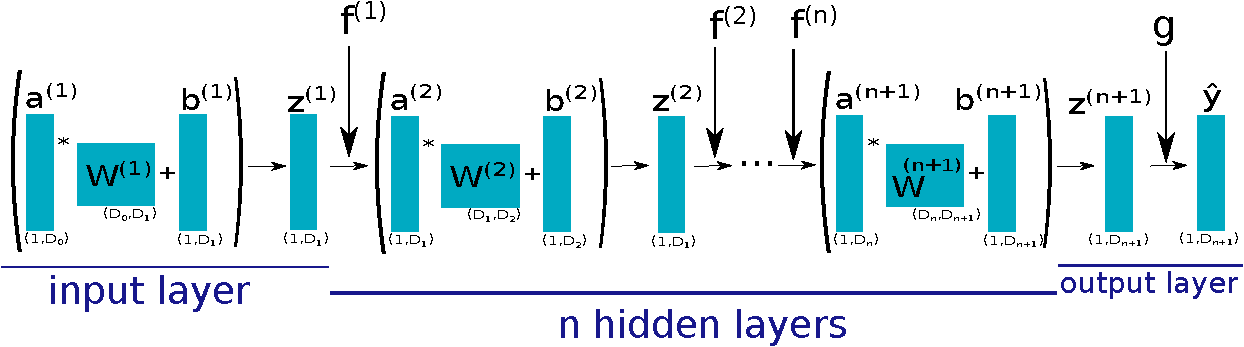
\includegraphics[scale=0.85]{abstrat_neural.pdf}
\end{center}
\caption{A neural network with $n$ hidden layers}
\label{abstract_neural}
\end{figure}
For $n\geq 1$, let $D_0, D_1, \dots, D_{n+1} \in \mathbb{N}$ (all grater than 0); let $f^{(1)}, \dots, f^{(n)} \mathbb{R}^{\mathbb{R}}$ be a sequence of non-linear functions; let $(x^1,y^1), \dots, (x^N,y^N)$ be the observations of a dataset (where $x^{d} \in \mathbb{R}^{D_{0}}$, and $y^{d} \in \mathbb{R}^{D_{n+1}}$;let $W^{(k)} \in \mathbb{R}^{D_{k-1},D_{k}}$  and $b^{(k)} \in \mathbb{R}^{D_{k}}$ for $k =1, \dots, n$. A neural network with $n$ hidden layers is a function applied to the observation $x^{d}$ from the dataset as follows:
\begin{equation}\label{eq:0}
a^{(1)} =x^{d}
\end{equation}
 \begin{equation}\label{eq:1}
z^{(k)}_{i} = \sum_{s=1}^{D_{(k-1)}}W^{(k)}_{s,i} a^{(k)}_{s} + b^{(k)}_{i}  \; {\small \text{ with }i = 1, \dots, D_{k} \text{ and }k = 1, \dots, n}
\end{equation}
\begin{equation}\label{eq:2}
a^{(k)} = f^{(k-1)}(z^{(k-1)})   \; {\small \text{ with }k = 2, \dots, n+1}
\end{equation}
\begin{equation}\label{eq:3}
\hat{y} = g(z^{(n+1)})
\end{equation}

The Figure \ref{abstract_neural} shows a visual representation of this model. We called \textbf{forward propagation} the calculation of $\hat{y}$. If we want to be explicit we should write $\hat{y}(W^{(1)}, \dots, W^{(n+1)},b^{(1)}, \dots, b^{(n+1)},x^{d})$, but to make things simple, we will only write $\hat{y}(x^{d})$. Let $Error$ be a function to measure the error between the hypothesis and the target, thus the error for a single observation is: 
\begin{equation}\label{eq:4}
J = Error(\hat{y}(x^{d}),y^{d})
\end{equation}
if we use regularization
\begin{equation}\label{eq:5}
J = Error(\hat{y}(x^{d}),y^{d}) + \sum_{k=1}^{n+1}\frac{1}{2}\lambda\sum_{i=1}^{D_{k-1}}\sum_{j=1}^{D_{k}}(W^{(k)}_{i,j})^{2}
\end{equation}
and for the whole dataset
\begin{equation}\label{eq:6}
J = \frac{1}{N}\sum_{d=1}^{N}(Error(\hat{y}(x^{d}),y^{d}) + \sum_{k=1}^{n+1}\frac{1}{2}\lambda\sum_{i=1}^{D_{k-1}}\sum_{j=1}^{D_{k}}(W^{(k)}_{i,j})^{2})
\end{equation}
To apply SGD we need to calculate the derivatives for each parameter $(W^{(1)}, \dots, W^{(n+1)},b^{(1)}, \dots, b^{(n+1)}$. The \textbf{back propagation algorithm} give us a easy method for doing that. We will compute error signals $\delta^{(2)}, \dots,\delta^{(n+2)}$ recursively in the reverse order as follows: 
\begin{equation}\label{eq:7}
\hat{y}(x^{d}) - y^{d} \; \; \footnote{This is not the general form, since it depends of the error function. To be honest, it is not clear to me if $\delta^{(n+2)}$ is $\frac{\partial J}{\partial \hat{y}}$ or $\frac{\partial J}{\partial  z^{n+1}}$}
\end{equation}
\begin{equation}\label{eq:8}
\delta^{(k)}_{j} = \sum_{s=1}^{D_{k}}\delta^{(k+1)}_{s}W^{(k)}_{j,s} {f^{\prime}}^{(k-1)} (a^{(k)}_{j})
\end{equation}
with $j = 1, \dots, D_{(k-1)}$  and $k = 2, \dots, n+1$.
\begin{equation}\label{eq:9}
\frac{\partial J}{\partial  W^{(k)}_{i,j}} = a^{(k)}_{i} \delta^{(k+1)}_{j}
\end{equation}
with $i = 1, \dots, D_{(k-1)}$, $j = 1, \dots, D_{(k)}$ and $k = 1, \dots, n+1$. If the cost function is \ref{eq:6}, then 
\begin{equation}\label{eq:10}
\frac{\partial J}{\partial  W^{(k)}_{i,j}} = a^{(k)}_{i} \delta^{(k+1)}_{j} + \lambda W^{(k)}_{i,j} 
\end{equation}
\begin{equation}\label{eq:11}
\frac{\partial J}{\partial  b^{(k)}_{j}} = \delta^{(k+1)}_{j} 
\end{equation}
with $j = 1, \dots, D_{(k)}$ and $k = 1, \dots, n+1$.

To make things simpler, we can simplify the equations (\ref{eq:8}),(\ref{eq:9}) and (\ref{eq:11}) using vector notation. For $A,B \in \mathbb{R}^{n,m}$ $A\circ B$ is the  Hadamard product, i.e., $(A\circ B)_{i,j} = A_{i,j}B_{i,j}$ . Similarly for $u,v \in \mathbb{R}^{n}$, $(v\circ u)_{i} = v_{i}u_{i}$. Hence,  

\begin{equation}\label{eq:8sim}
\bm{\delta^{(k)} = (\delta^{(k+1)} {(W^{(k)})}^{T}) \circ {f^{\prime}}^{(k-1)} (a^{(k)})}
\end{equation}

\begin{equation}\label{eq:9sim}
\bm{\frac{\partial J}{\partial  W^{(k)}} = {a^{(k)} \delta^{(k+1)}}^{T}}
\end{equation}

\begin{equation}\label{eq:11sim}
\bm{\frac{\partial J}{\partial  b^{(k)}} =  \delta^{(k+1)}}
\end{equation}

\pagebreak

\section{Example}

\begin{figure}
\begin{center}
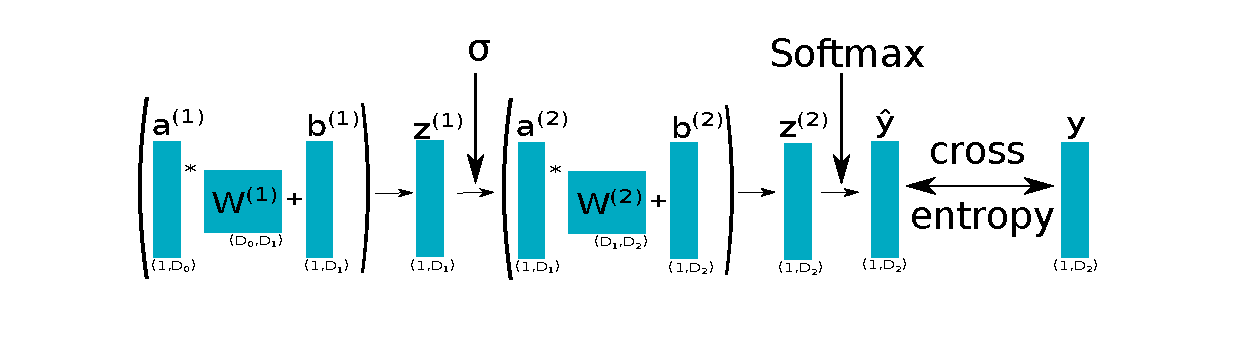
\includegraphics[scale=0.85]{example.pdf}
\end{center}
\caption{A neural network with $1$ hidden layer}
\label{example}
\end{figure}
Figure \ref{example} shows a neural network with a single hidden layer. The only non-linear function is the sigmoid function $\sigma$ and the function in the output layer is the sigmoid function. As a error measure we use cross entropy, assuming $y \in \mathbb{R}^{D_2}$ is an one-hot vector. Hence
\begin{equation}\label{eq:12}
z^{(1)}_i = \sum_{s=1}^{D_{x}}W^{(1)}_{s,i} x_{s} + b^{(1)}_{i}  \; {\small \text{ with }i = 1, \dots, D_{1}}
\end{equation}
\begin{equation}\label{eq:13}
a^{(2)}_i = \sigma(z^{(1)}_i )  \; {\small \text{ with }i = 1, \dots,D_{1}}
\end{equation}
\begin{equation}\label{eq:14}
z^{(2)}_j = \sum_{s=1}^{D_{1}}W^{(2)}_{s,j} a^{(2)}_{s} + b^{(2)}_{j} \;\; {\small \text{ with }j = 1, \dots, D_{2}}
\end{equation}
\begin{equation}\label{eq:15}
\hat{y}_j = softmax(z^{(2)}_j) \;\; {\small \text{ with }j = 1, \dots, D_{2}}
\end{equation}
\begin{equation}\label{eq:16}
J(y,\hat{y}) = CE(y,\hat{y}) = -\sum_{s=1}^{D_{2}} y_s  \log(\hat{y}_s)
\end{equation}
where CE stands for \textit{cross-entropy}.

Note that $\frac{\partial J}{\partial  z^{(2)}} = \hat{y} - y$. So taking $\delta^{(3)} = \hat{y} - y$, we can apply the back propagation algorithm.

For $i \in {1,\dots,D_{1}}$ and $j \in {1,\dots,D_{2}}$ we have
\begin{align*}
\frac{\partial J}{\partial W^{(2)}_{i,j}} & = a^{(2)}_{i}\delta^{(3)}_{j}\\
& = a^{(2)}_{i}(\hat{y}_{j} - y_{j})\; .
\end{align*}
\begin{align*}
\frac{\partial J}{\partial b^{(2)}_{j}} & = \delta^{(3)}_{j}\\
& = (\hat{y}_{j} - y_{j})\; .
\end{align*}

For $j \in {1,\dots,D_{1}}$ we have
\begin{align*}
\delta^{(2)}_{j} & = \sum_{s=1}^{D_{2}}\delta^{(3)}_{s}W^{(2)}_{j,s} \sigma^{\prime} (a^{(2)}_{j})\\
& = \sum_{s=1}^{D_{2}}(\hat{y}_{s} - y_{s})W^{(2)}_{j,s}\sigma^{\prime} (a^{(2)}_{j})\; .
\end{align*}

For $i \in {1,\dots,D_{0}}$ and $j \in {1,\dots,D_{1}}$ we have
\begin{align*}
\frac{\partial J}{\partial W^{(1)}_{i,j}} & = a^{(1)}_{i}\delta^{(2)}_{j}\\
& = a^{(1)}_{i}\sum_{s=1}^{D_{2}}(\hat{y}_{s} - y_{s})W^{(2)}_{j,s}\sigma^{\prime} (a^{(2)}_{j})\; .
\end{align*}
\begin{align*}
\frac{\partial J}{\partial b^{(1)}_{j}} & = \delta^{(2)}_{j}\\
& = \sum_{s=1}^{D_{2}}(\hat{y}_{s} - y_{s})W^{(2)}_{j,s}\sigma^{\prime} (a^{(2)}_{j})\; .
\end{align*}
\end{document}
